
\subsection{\texorpdfstring{$\ttbar$}{h1} and\texorpdfstring{$~\ttbar$}{h2}-like backgrounds}
\label{Sec:emuSS}

The background for electrons coming from \ttbar\ and \ttbar-like processes is estimated directly from MC simulation.

As we know, all these processes are flavour-symmetric and the branching ratio to e$\mu$ is twice larger than the branching ratio to ee for all these processes. Because of that the e-$\mu$ invariant mass spectrum provides an excellent control region to validate the MC predictions for these processes. This validation is described below.
%The contribution of these backgrounds to the e$^{-}$ e$^{+}$ spectrum is estimated from Monte-Carlo
%simulations after having checked that the simulations describe the sample of $e\mu$ events well.
In order to study the e-$\mu$ mass spectrum, we use the SingleMuon datasets and the ``HLT\_Mu50'' trigger is applied on data events.
The electron-muon events are selected such that the first object is a global muon passing the high \pt muon identification criteria \cite{CMS-AN-2016-391},
and the second object is an electron passing the HEEP ID selection. Electron is required to have $\pt>35~\mathrm{GeV}$ while muon is required $\pt>60~\mathrm{GeV}$.
Since high energetic muons can produce bremsstrahlung with an associated super-cluster in the ECAL in the direction of the muon's
inner track, the selected muons can lead to fake electron candidates. Therefore, an electron veto is applied such that if there is
a global muon with $\pt > 5$ GeV within $\Delta R <0.1$ of the electron, the electron is not selected. Finally the electron and muon should have opposite sign.
The Monte Carlo samples and the cross-sections used are documented in Table~\ref{tab:Z_mc-samples_1}, all scale factors have been applied to MC events.

The estimation of the multi-jet background from simulated samples is not feasible because of the small misreconstruction rate for the jets.
Instead, the multi-jet background is obtained from the same sign e$\mu$ spectrum, where the electron and muon have the same charge.
The contributions of the other SM processes (estimated from simulations) are subtracted from the data
spectrum in same sign e$\mu$ spectrum and the remaining spectrum is taken to come from multi-jet events. For the multi-jet background, the spectrum for the same sign or opposite sign e$\mu$ pair should be the same.


The invariant mass spectra of e$\mu$ events in data and MC are shown for both datasets in Figure \ref{fig:ttbaremu}.

%=================================================
\begin{figure}[!htb]
\begin{center}
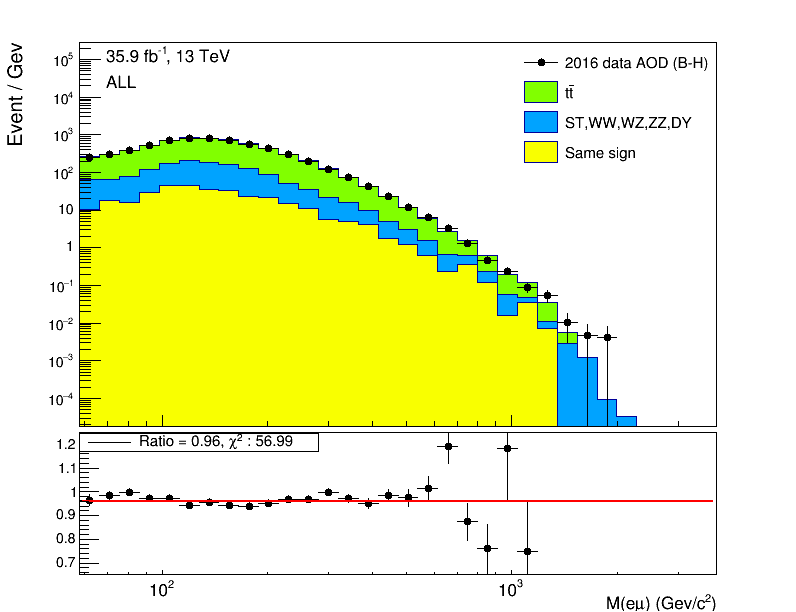
\includegraphics[angle=0,width=0.47\textwidth]{figures/Zprime/2016/bkg_ttbar/SS/hratio_M_emu1__ALL.png}
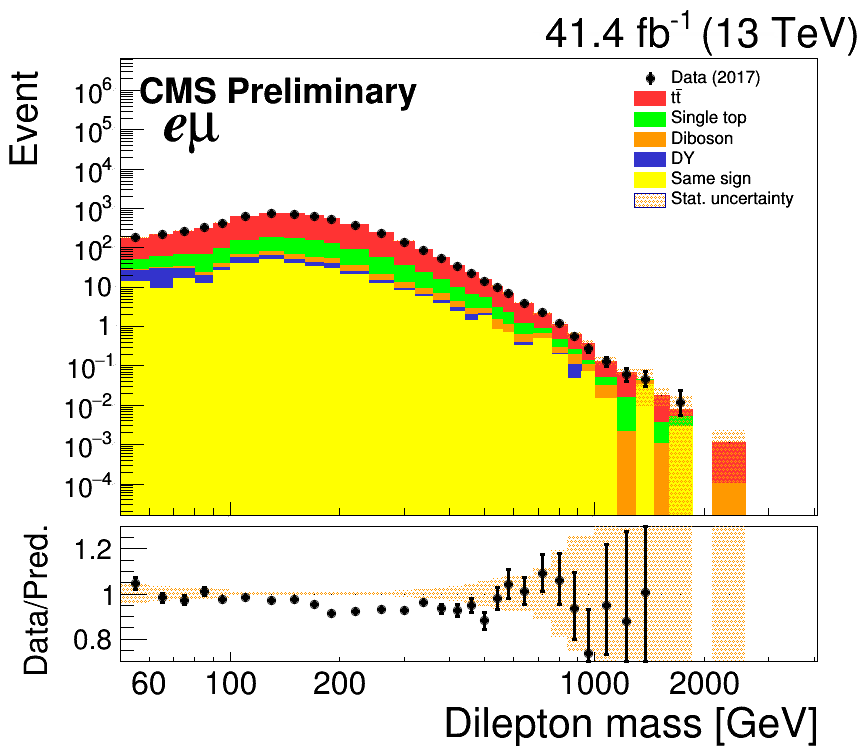
\includegraphics[angle=0,width=0.47\textwidth]{figures/Zprime/2017/bkg_ttbar/SS/ALL_hratio_M_emu_massDep.png}
\caption{Invariant mass spectra of the e$\mu$ events in data and MC for 2016 (left) \cite{CMS-AN-2016-404} and 2017 (right) \cite{CMS-AN-2018-021}.}
\label{fig:ttbaremu}
\end{center}
\end{figure}
%=================================================

After having checked that the simulations describe the sample of e$\mu$ events well, the
contribution of these backgrounds to the ee spectrum is estimated from Monte Carlo. The tendency of the data/MC ratio to decrease at high mass come from a known effect from a misdescription of the top \pt in the \ttbar simulation samples (from higher order corrections), which is not taken into account in the above plots.


